\subsection{Comparison with existing pseudoscalar models and recasting of HF+\MET search results}
\label{sub:DMHF_rescaling}

To date, simplified models of DM~\cite{Abercrombie:2015wmb,Backovic:2015soa} that add a single scalar or pseudoscalar mediator and the DM particle to the SM are used as benchmarks for the Run II CMS and ATLAS HF+\MET searches. These are called \texttt{DMsimp} models in the following. The kinematics and cross-section of the pseudoscalar \texttt{DMsimp} models can map directly onto those of the 2HDM+a model, when accounting for the contributions from the light and heavy pseudoscalar mediators.

%with $\mathrm{M_{a}}=100$ GeV 

\begin{figure}
  \centering
  \begin{subfigure}[b]{0.6\textwidth}
    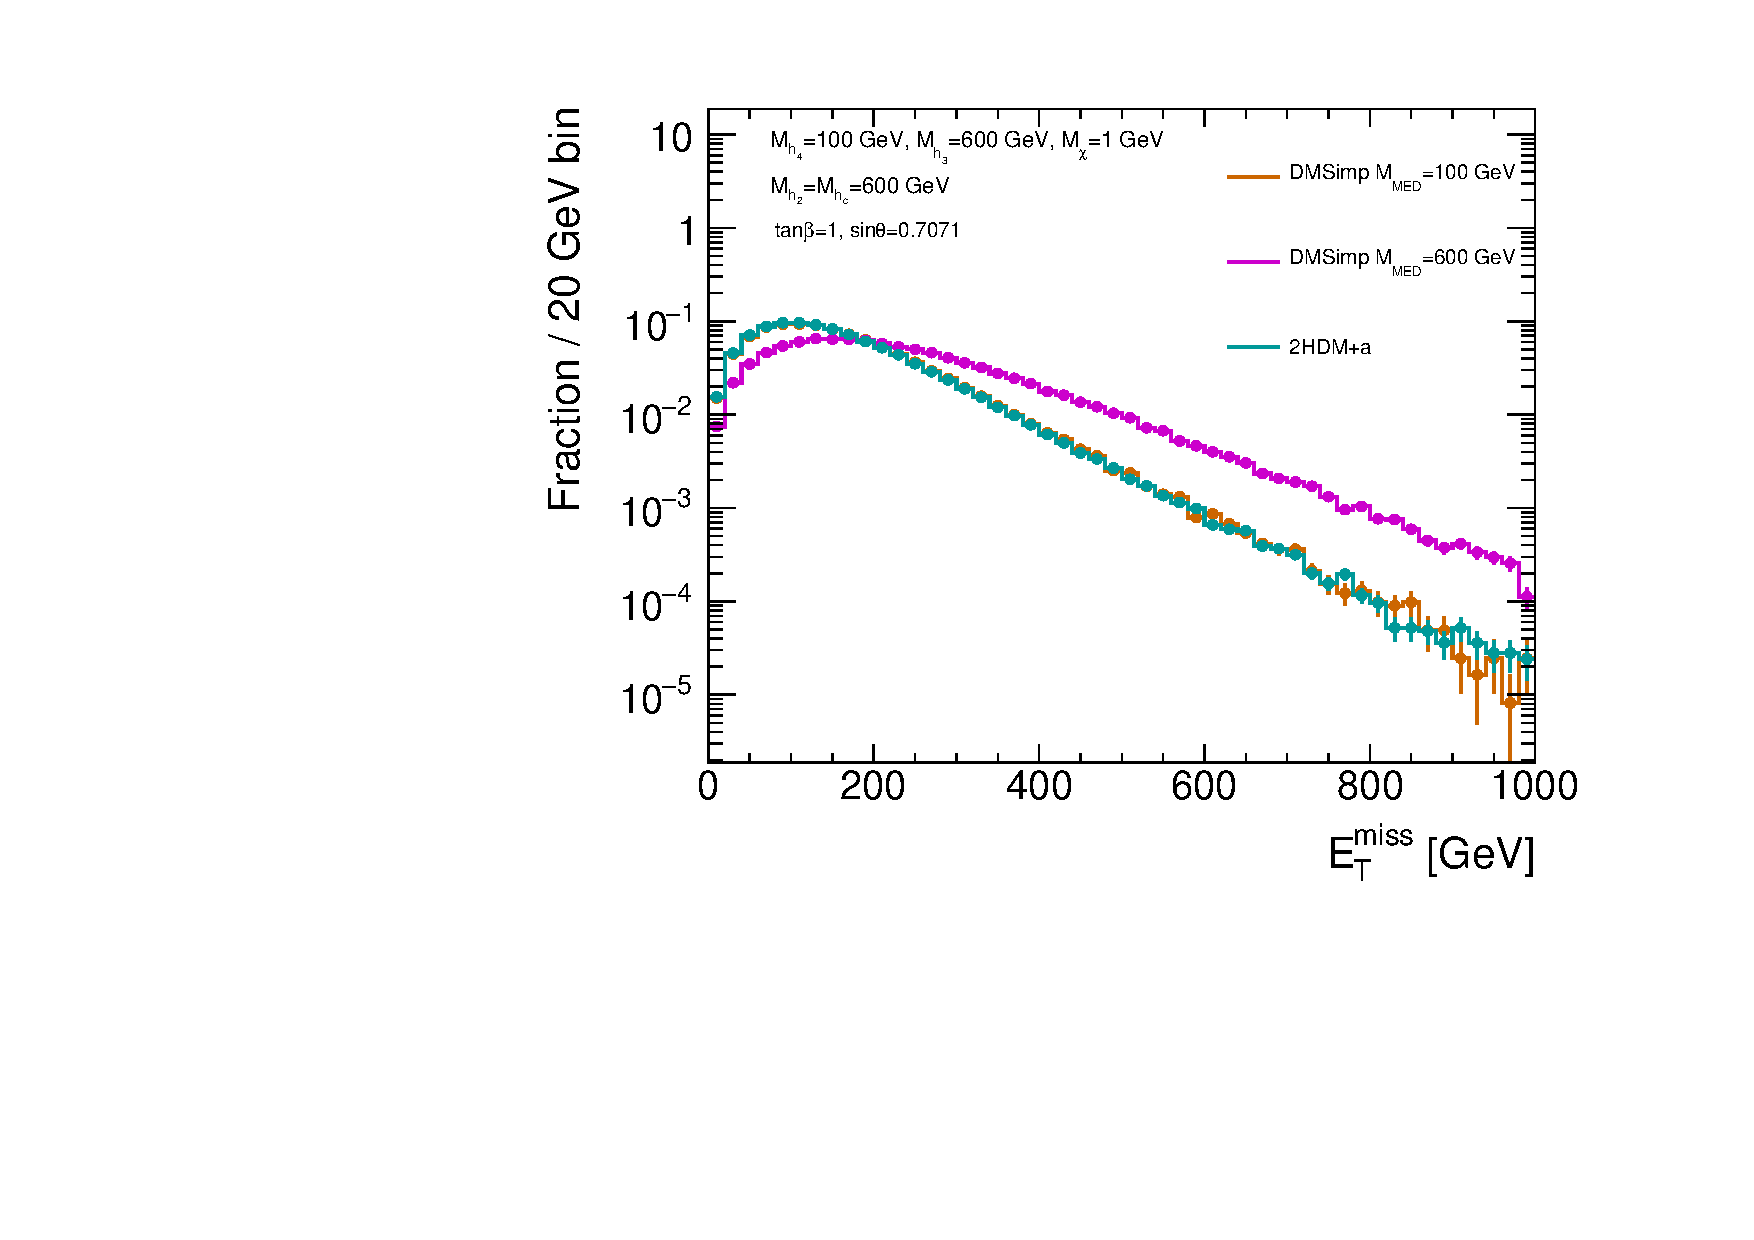
\includegraphics[width=\textwidth]{texinputs/04_grid/figures/DMHF/benchmarking/MDM_1_Ma_100_MA_600_sinp_0.7071_tanb_1.0_VS_DMSimp_100_600_Decayed/metlog.pdf}
    \caption{$E_{T}^{miss}$}
  \end{subfigure}\\
  \begin{subfigure}[b]{0.45\textwidth}
    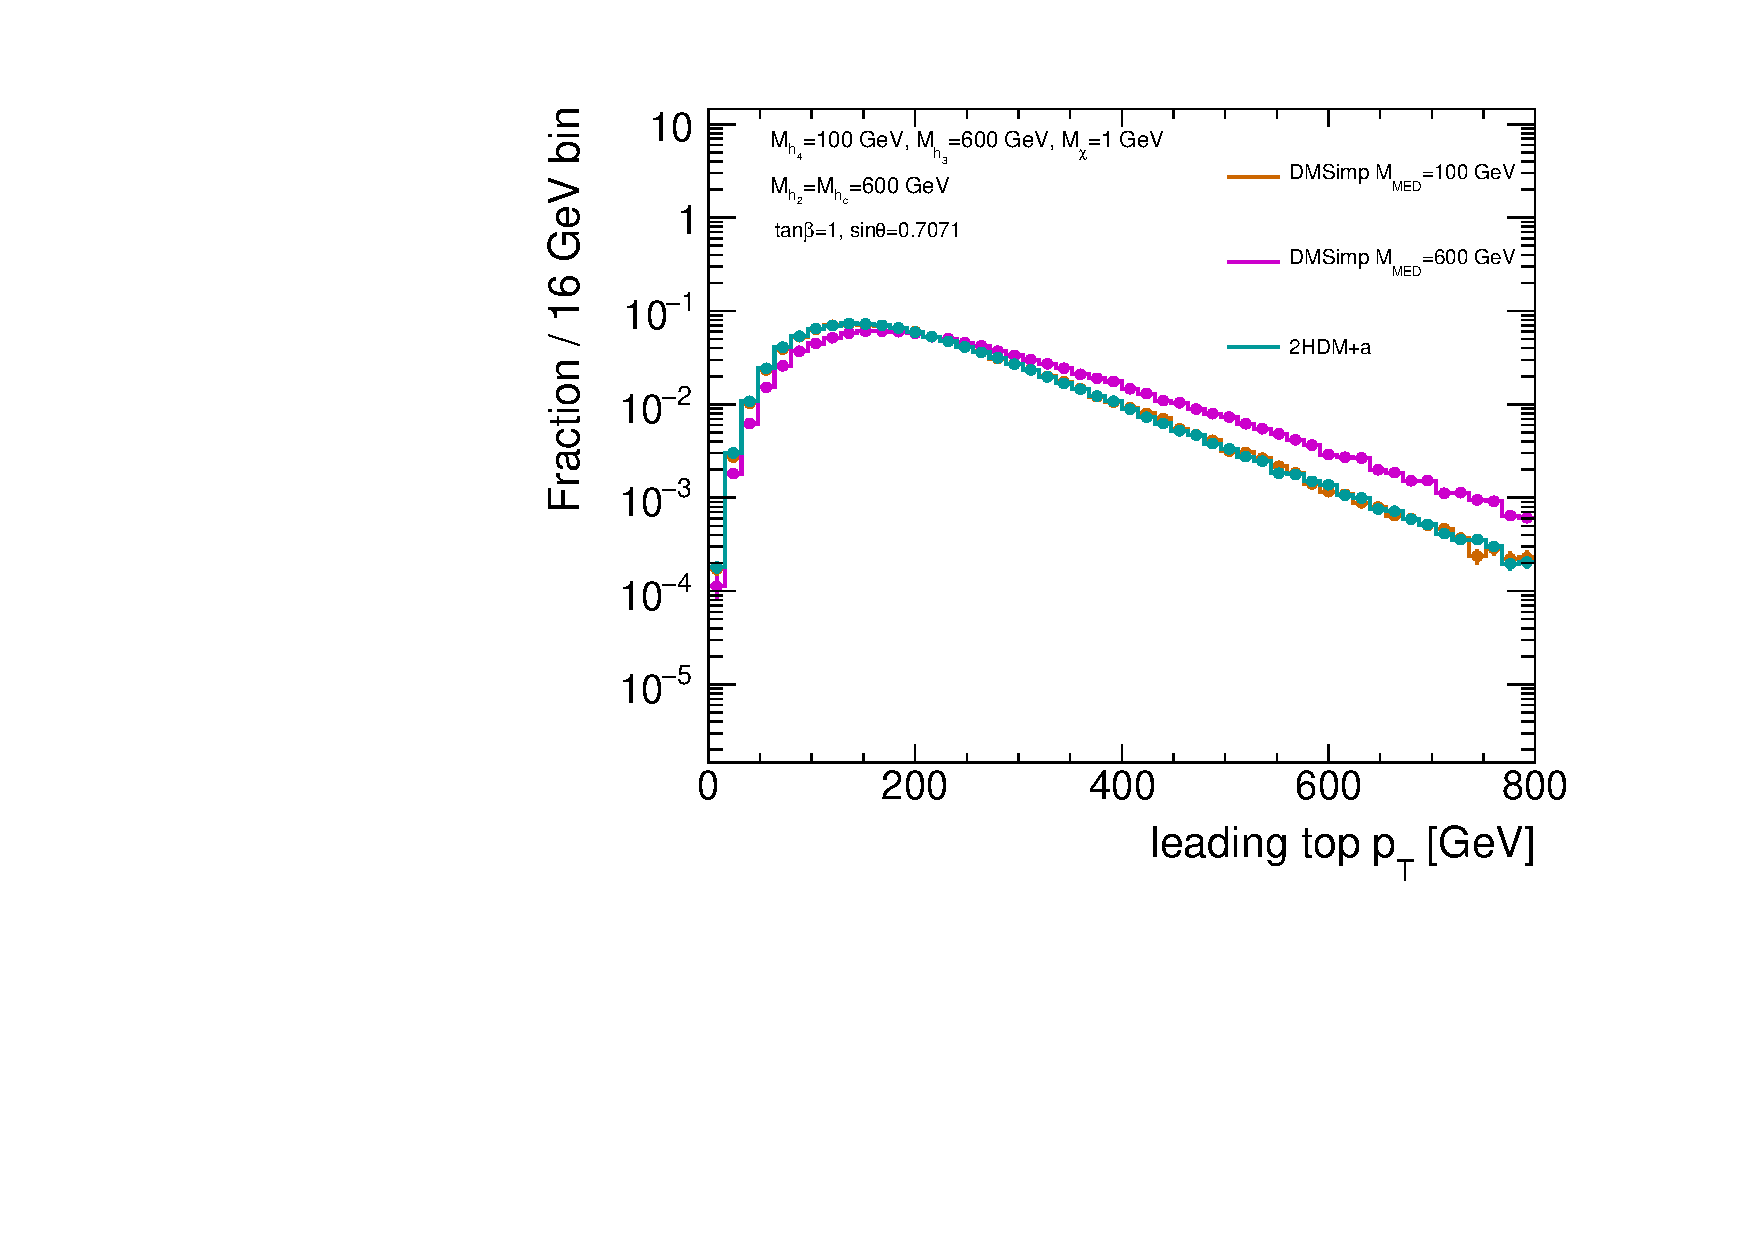
\includegraphics[width=\textwidth]{texinputs/04_grid/figures/DMHF/benchmarking/MDM_1_Ma_100_MA_600_sinp_0.7071_tanb_1.0_VS_DMSimp_100_600_Decayed/top1ptlog.pdf}
    \caption{Leading top $p_{T}$}
  \end{subfigure} 
  \begin{subfigure}[b]{0.45\textwidth}
    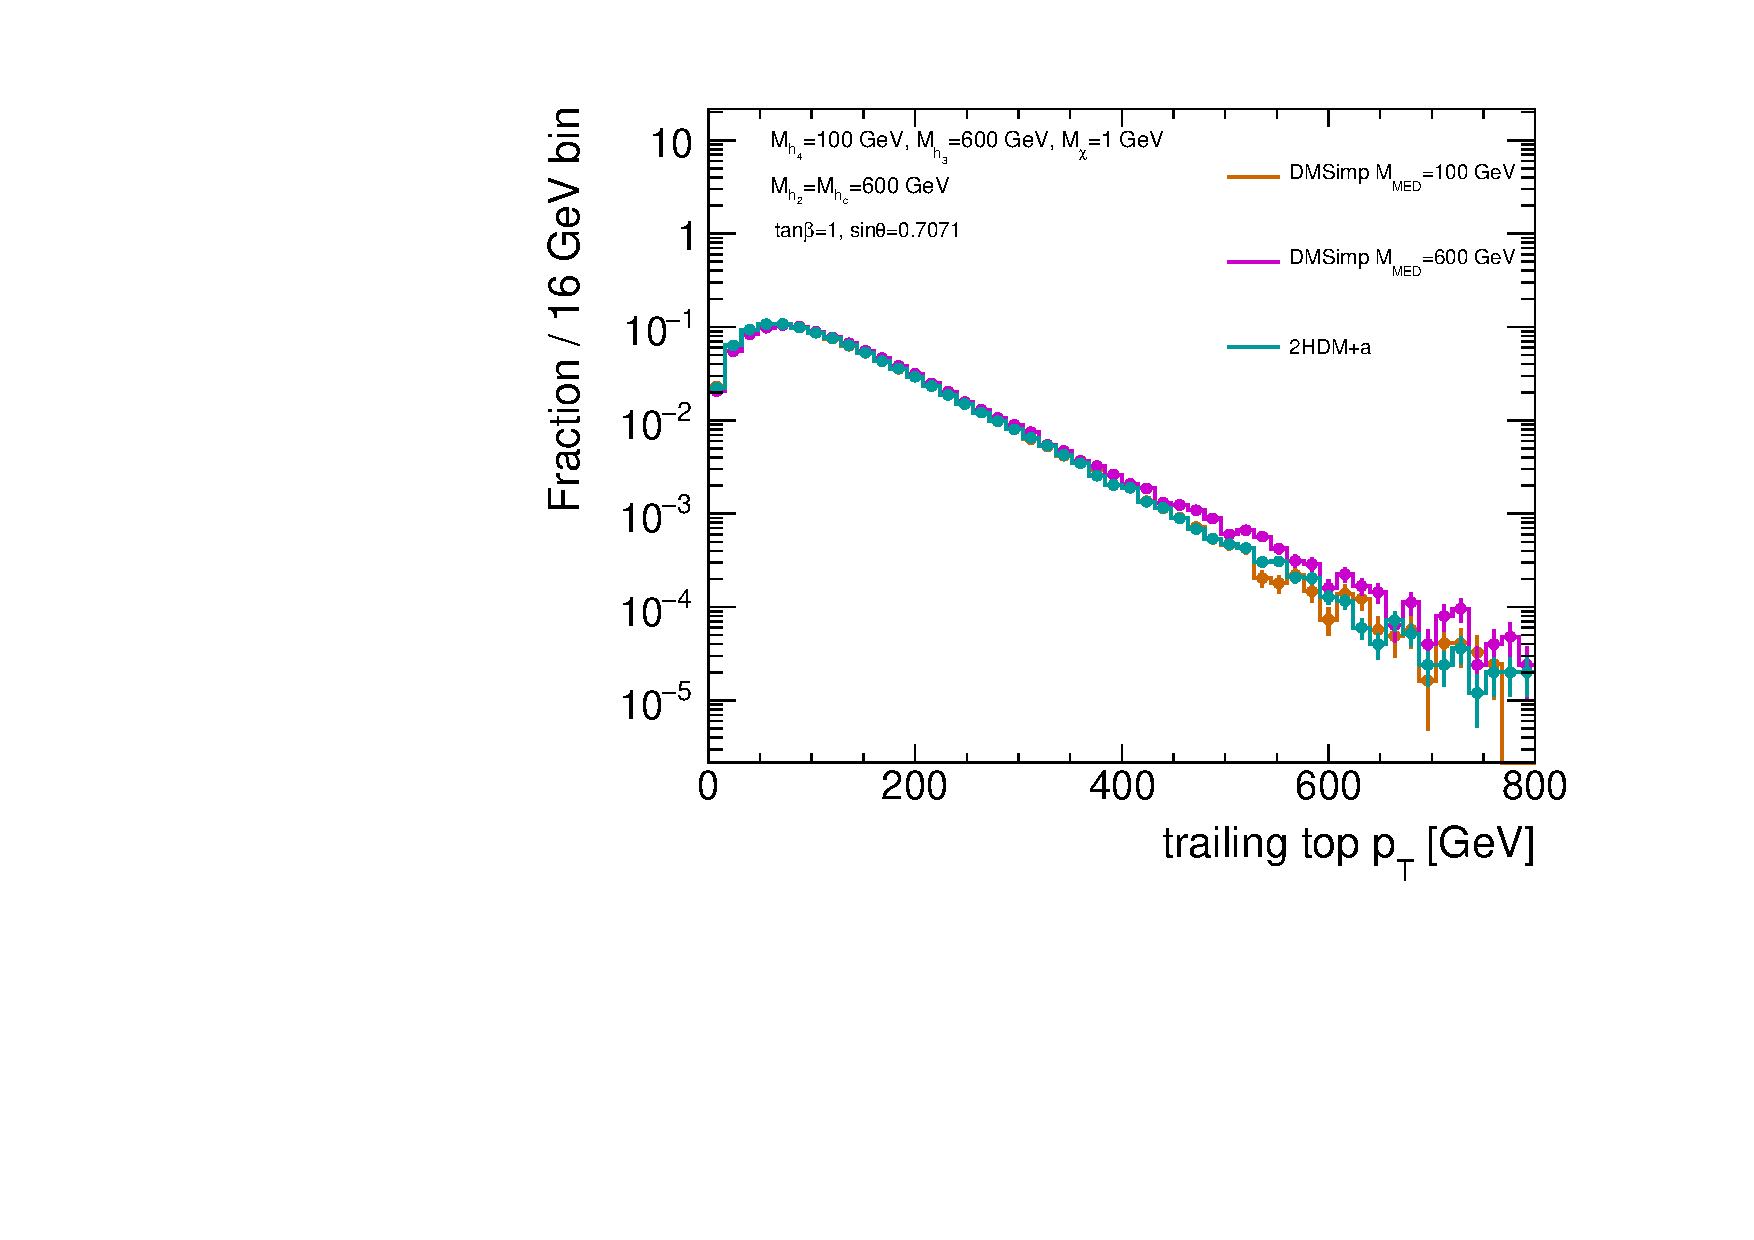
\includegraphics[width=\textwidth]{texinputs/04_grid/figures/DMHF/benchmarking/MDM_1_Ma_100_MA_600_sinp_0.7071_tanb_1.0_VS_DMSimp_100_600_Decayed/top2ptlog.pdf}
    \caption{Trailing top $p_{T}$}
  \end{subfigure}
  \caption{The $E_{T}^{miss}$, leading and trailing top $p_{T}$ distributions for inclusive $t\bar{t}+\chi\bar{\chi}$ production for different values of $\mathrm{M_a}$, with $\mathrm{M_A}=\mathrm{M_H}=\mathrm{M_{H^{\pm}}}=600$ GeV, $\tan\beta=1$, \mDM=1 GeV and $\sin\theta=0.7071$, compared to the \texttt{DMsimp} pseudoscalar model.}
  \label{fig:kin_DMSimpV2HDMa}
\end{figure}

%Not sure this figure can be added, maybe appendix?
%\begin{figure}
%  \centering    
%  \begin{subfigure}[b]{0.49\textwidth}
%    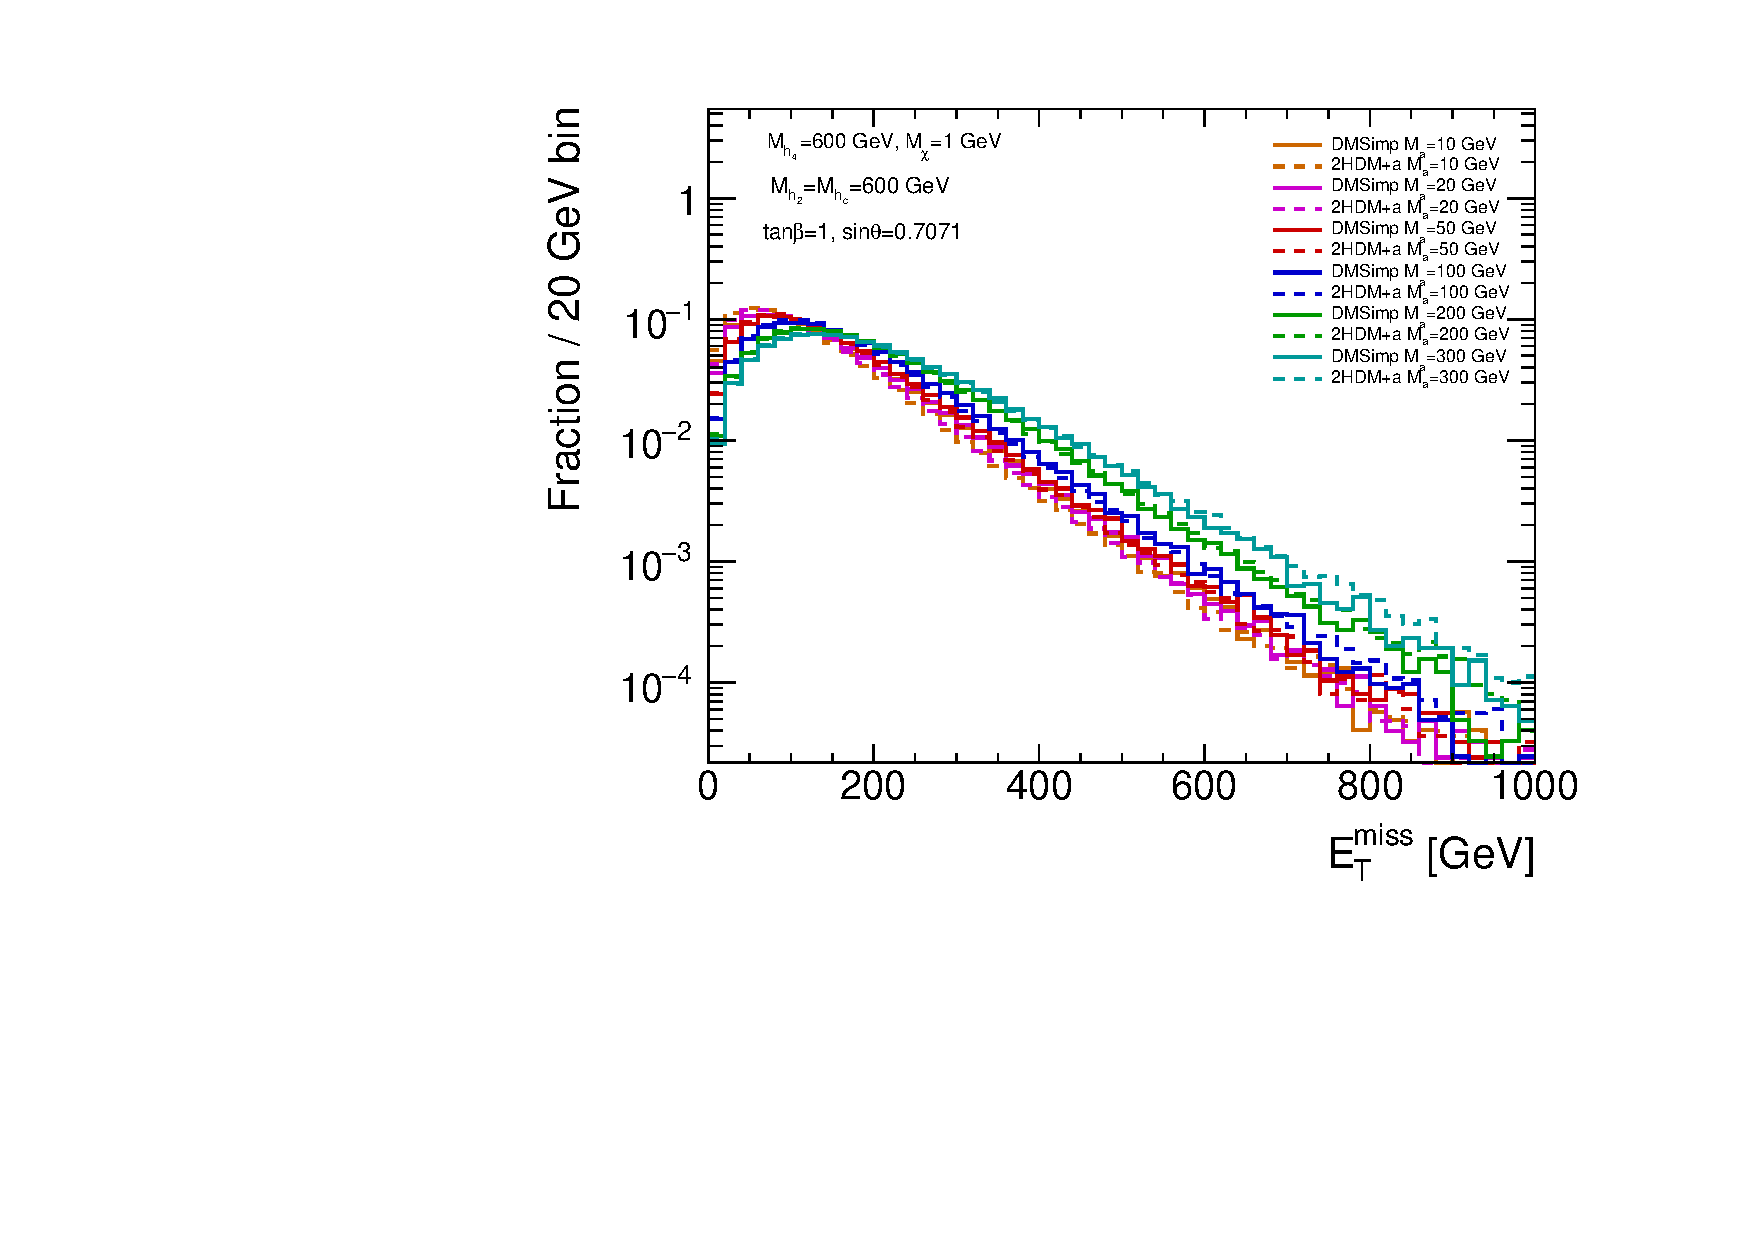
\includegraphics[width=\textwidth]{texinputs/04_grid/figures/DMHF/benchmarking/MDM_1_MA_600_sinp_0.7071_tanb_1.0_DMsimpV2HDMa/metlog.pdf}
%    \caption{$E_{T}^{miss}$}
%  \end{subfigure}
%  \begin{subfigure}[b]{0.49\textwidth}
%    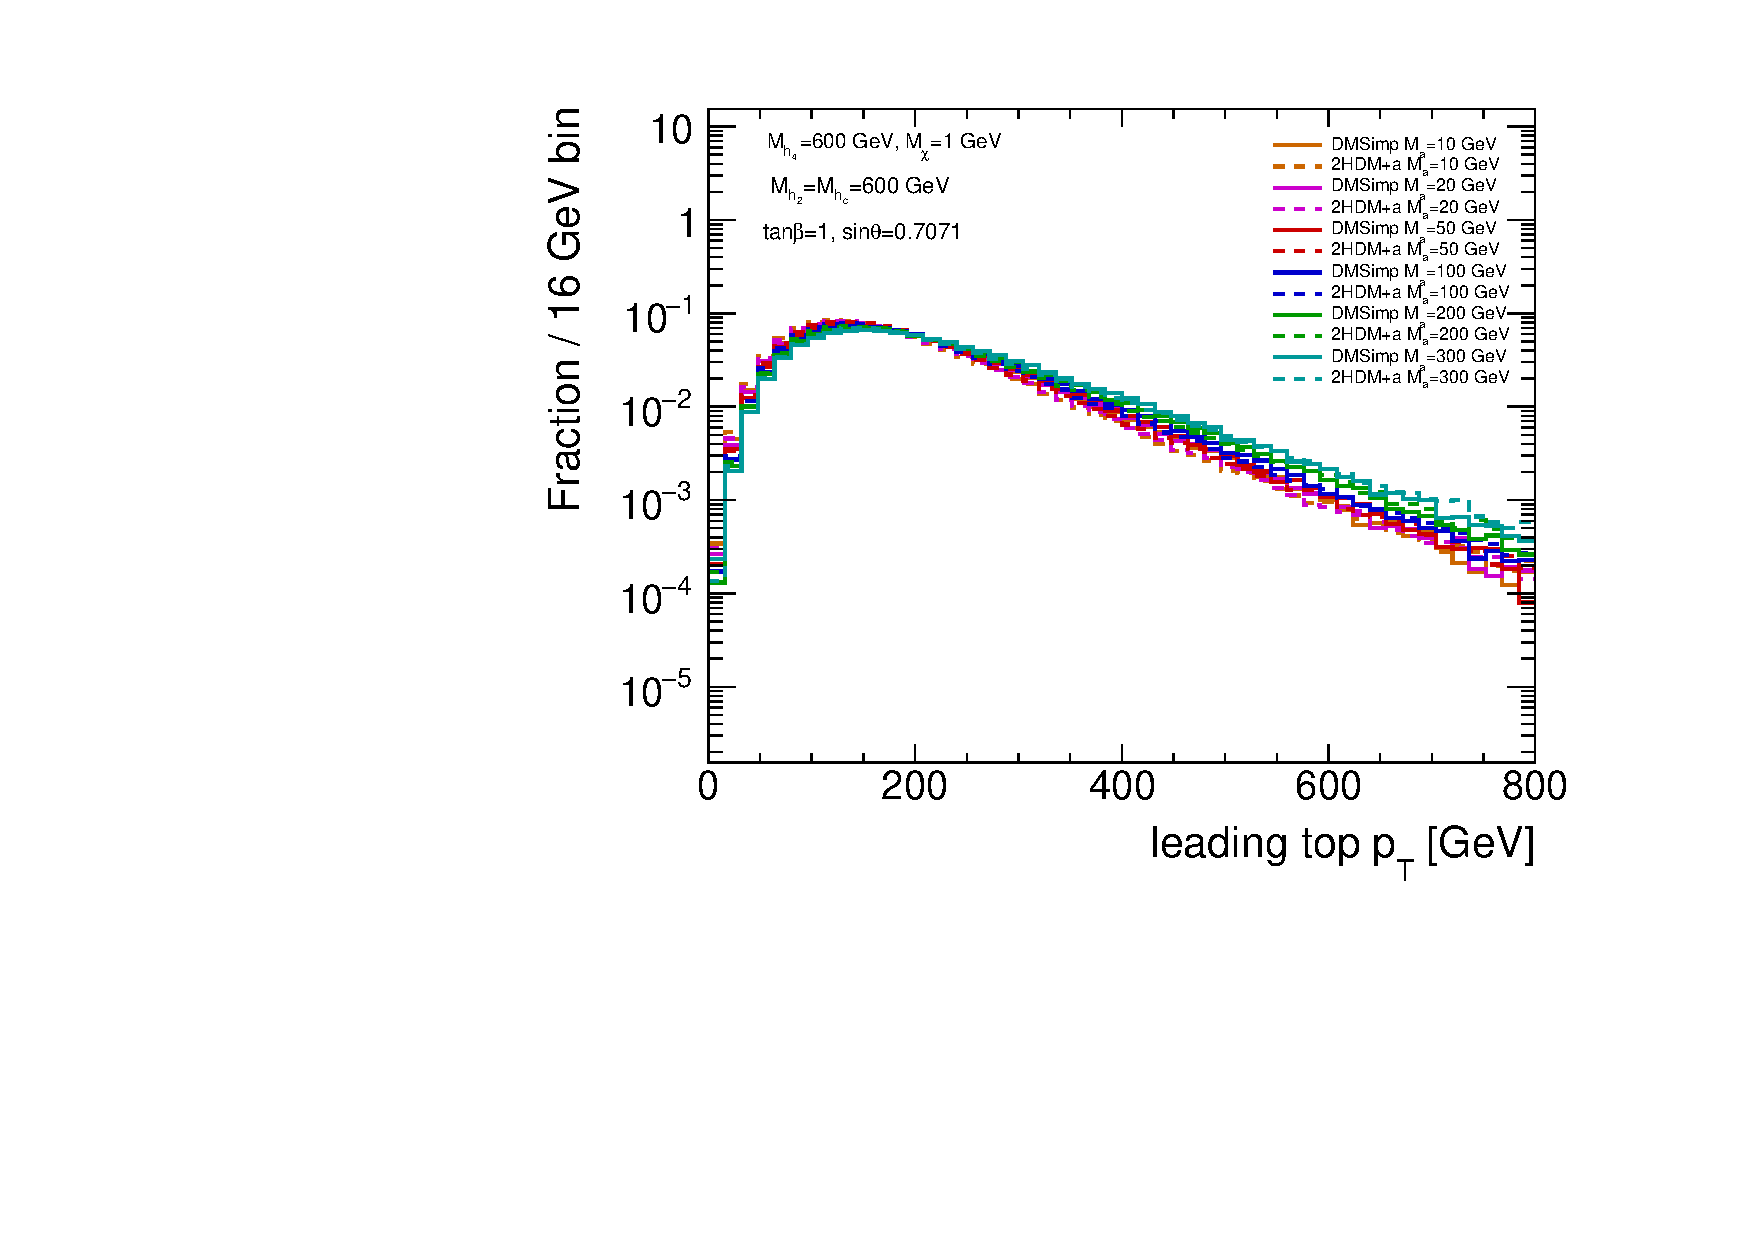
\includegraphics[width=\textwidth]{texinputs/04_grid/figures/DMHF/benchmarking/MDM_1_MA_600_sinp_0.7071_tanb_1.0_DMsimpV2HDMa/top1ptlog.pdf}
%    \caption{Leading top $p_{T}$}
%  \end{subfigure} \\
%  \begin{subfigure}[b]{0.49\textwidth}
%    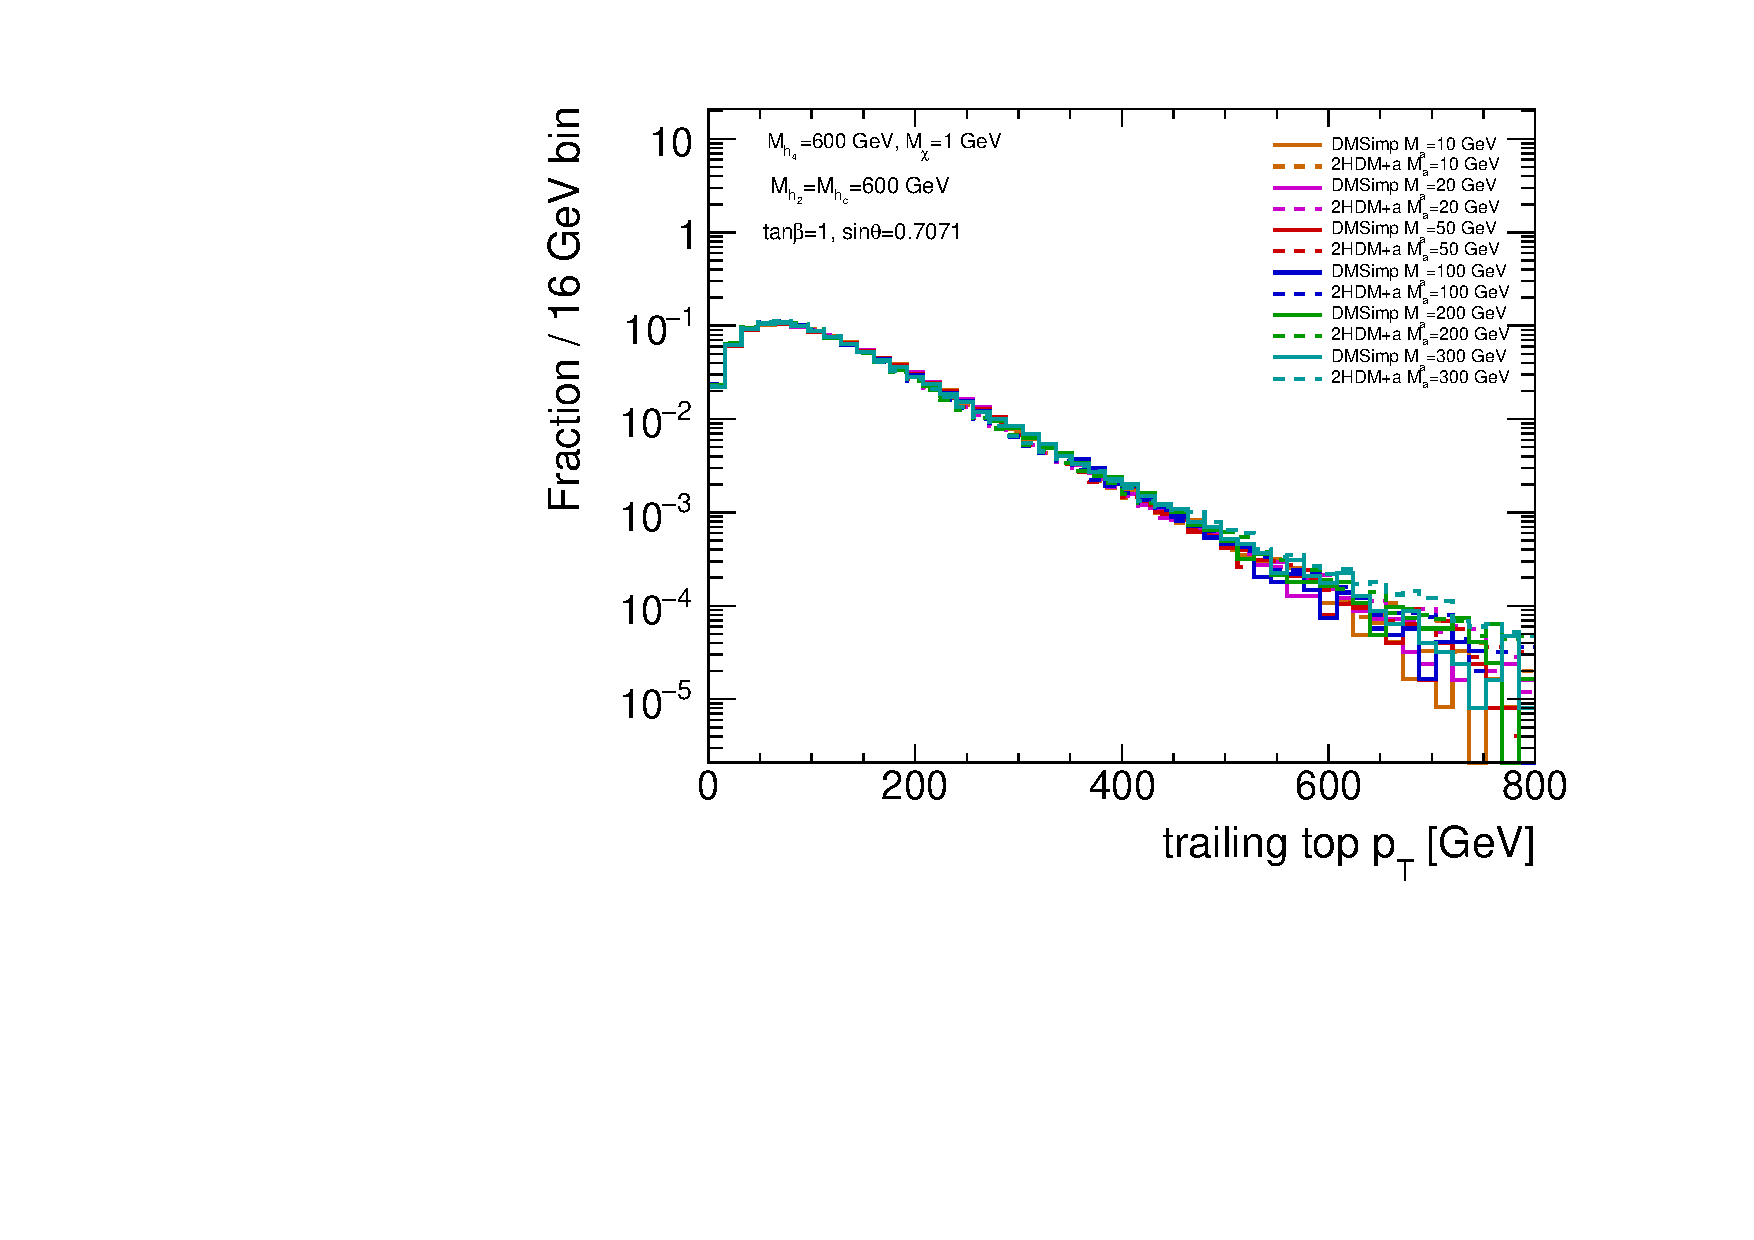
\includegraphics[width=\textwidth]{texinputs/04_grid/figures/DMHF/benchmarking/MDM_1_MA_600_sinp_0.7071_tanb_1.0_DMsimpV2HDMa/top2ptlog.pdf}
%    \caption{Trailing top $p_{T}$}
%  \end{subfigure}
%  \caption{The $E_{T}^{miss}$, leading and trailing top $p_{T}$ distributions for inclusive $t\bar{t}+\chi\bar{\chi}$ production generated from the \texttt{DMsimp} (solid) and the 2HDM+a (dashed) models with various values of $\mathrm{M_a}$. The 2HDM+a models are generated with the following model parameters:$\mathrm{M_A}=600$ GeV, $\mathrm{M_H}=\mathrm{M_{H^{\pm}}}=600$ GeV, $\tan\beta=1$, and $\sin\theta=0.7071$.}
%\label{fig:DMSimpV2HDMa}
%\end{figure}

\begin{figure}
  \centering
  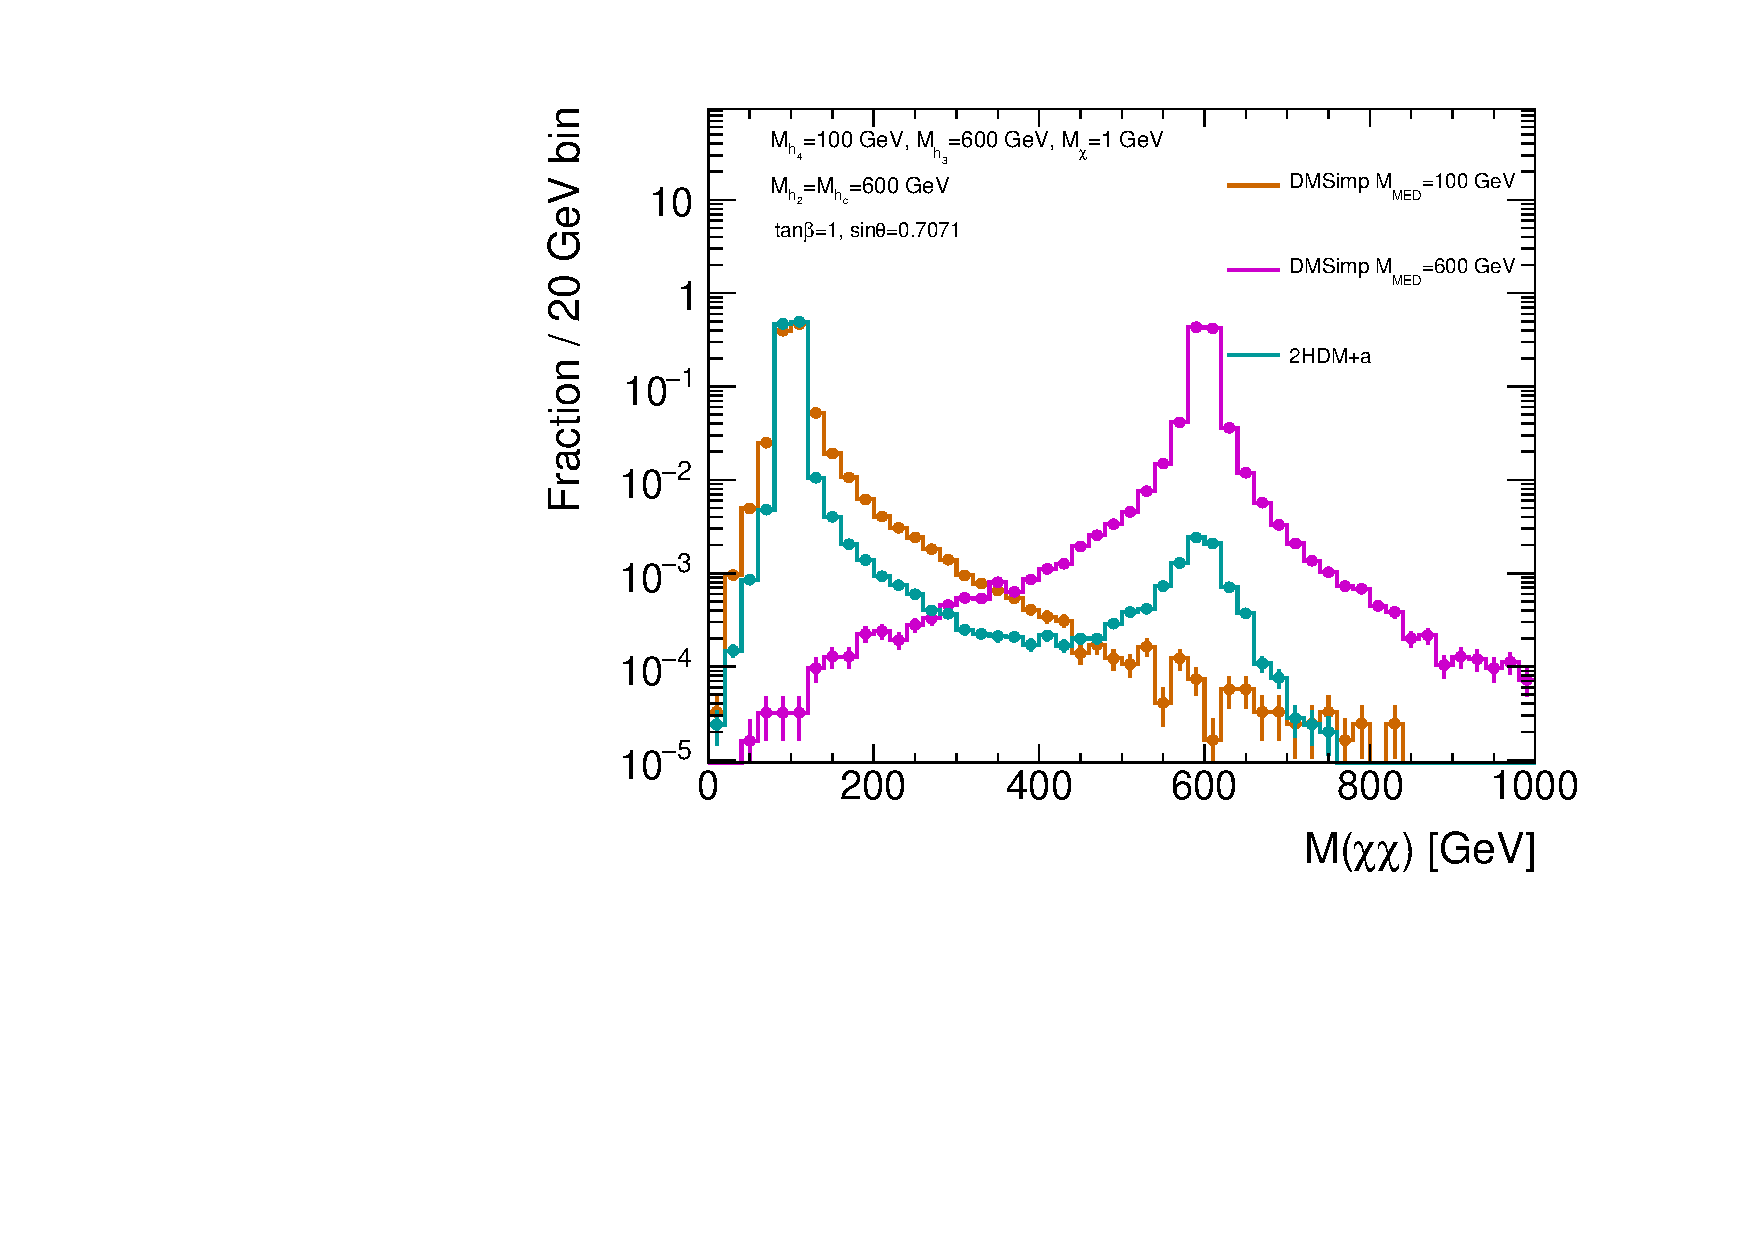
\includegraphics[width=0.6\textwidth]{texinputs/04_grid/figures/DMHF/benchmarking/MDM_1_Ma_100_MA_600_sinp_0.7071_tanb_1.0_VS_DMSimp_100_600_Decayed/mchichi.pdf}
  \caption{The mass distribution of the $\chi\bar{\chi}$ system for \texttt{DMsimp} pseudoscalar models with $\mathrm{M_a}=100$ GeV and $\mathrm{M_a}=600$ GeV, compared with 2HDM+a with $\mathrm{M_a}=100$ GeV, $\mathrm{M_A}=600$ GeV, $\mathrm{M_H}=\mathrm{M_{H^{\pm}}}=600$ GeV, $\sin\theta=0.7071$ and $\tan\beta=1$. TODO: needs different markers.}
  \label{fig:mchichi_DMsimpV2HDMa}
\end{figure}

The comparison of some of the relevant kinematic distributions between the pseudoscalar simplified model and the 2HDM+a model using two different values of $\mathrm{M_{a}}$, is shown in \autoref{fig:kin_DMSimpV2HDMa}. In these figures, the parameters used are: $\mathrm{M_{A}}=600$ GeV, $\mathrm{M_{H}}=\mathrm{M_{H^{\pm}}}=600$ GeV, $\sin\theta=0.7071$, $\tan\beta=1$, while $\mathrm{M_{a}}$ is either 100 or 600 GeV. The distributions for the two models agree when the mediator mass in the \texttt{DMsimp} model is set to \ma and the contribution from $A$ decays is smaller since $A$ is more massive than $a$.

\begin{figure}[htb]
\begin{center}
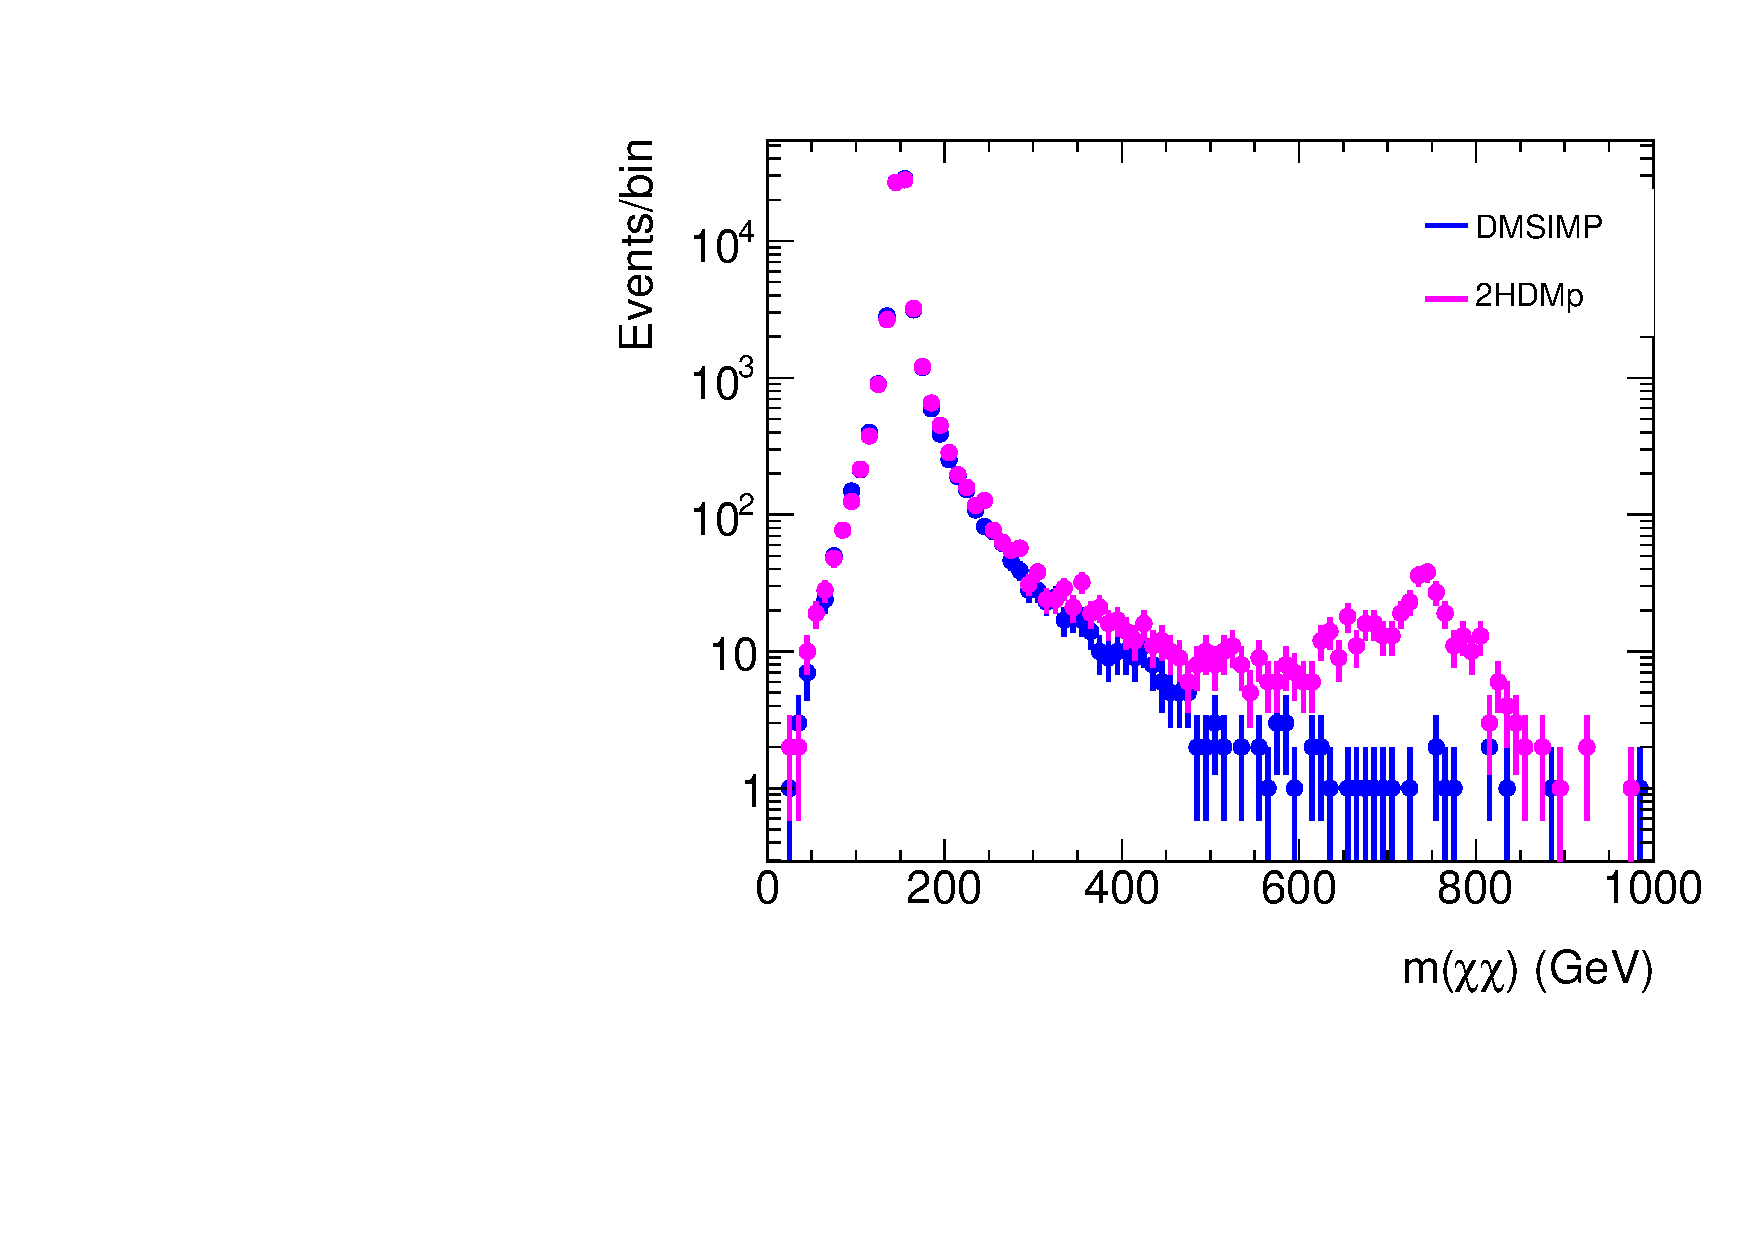
\includegraphics[width=0.48\textwidth]{texinputs/04_grid/figures/DMHF/mdd150.pdf}
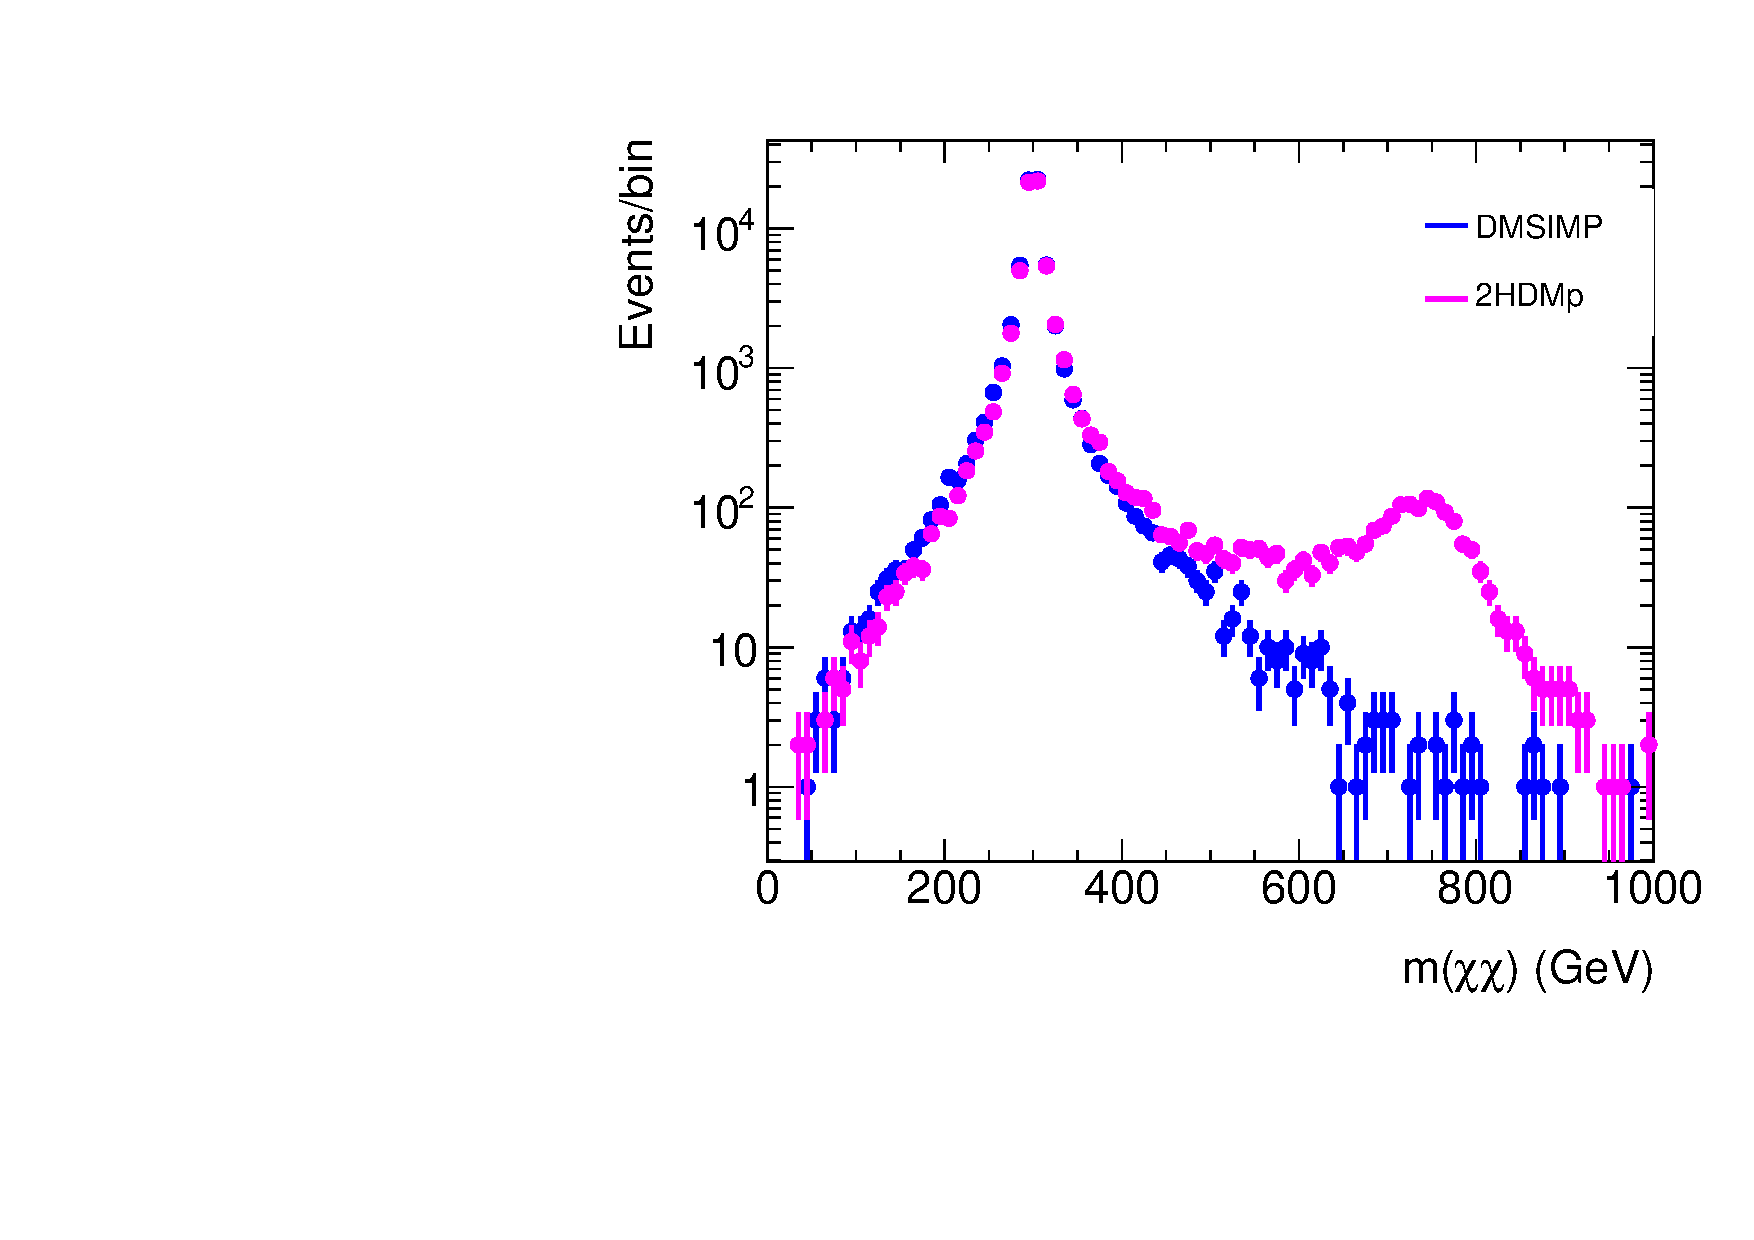
\includegraphics[width=0.48\textwidth]{texinputs/04_grid/figures/DMHF/mdd300.pdf}
\caption{Comparison of $m(\chi\chi)$, the invariant mass of 
the two DM particles for the \texttt{DMSimp} (blue) and the $2HDMp$ model (magenta) with $m(A) = M_{med} = 750$ GeV. The plot on the left uses \ma=150 GeV, while the plot on the right uses \ma=300 GeV.}
\label{fig:mdd}
\end{center}
\end{figure}

The \texttt{DMSimp} model has only one mediator particle. \autoref{fig:mchichi_DMsimpV2HDMa} shows that the 2HDM+a model can be represented as the sum of two contributions, one from the light pseudoscalar and the other one from the heavy pseudoscalar. This is because the HF+\MET signatures are dominantly produced in diagrams involving the invisible decays of the two CP-odd scalars. The 2HDM+a model is equivalent to the single pseudoscalar simplified model \texttt{DMsimp} when $A$ is much heavier than $a$, and therefore the former does not contribute to the considered final state. However, when the two mediators are closer in mass, the $pp\rightarrow ttA$ contribution becomes more relevant. This can be seen in Figure~\ref{fig:mdd}, where the two models are compared assuming $m(A) = 750$ GeV and two different values for $m(a)$. An excellent agreement is observed between \texttt{DMsimp} and 2HDM+a at parton-level variables sensitive to the helicity structure of the interaction between top and the mediator\cite{Haisch:2016gry}, if the invariant mass of the two DM particles in the 2HDM is smaller than 200(300)~GeV for $m(a)=150(300)$~GeV respectively. This gives confidence that, once the contribution from $A$ production is identified and separated, it is possible to fully map the $2HDM+a$ kinematics to the existing \texttt{DMsimp} model. 


% and \autoref{fig:mchichi_DMsimpV2HDMa} why different in chichi and similar in MET

%In Fig.~\ref{fig:DMSimpV2HDMa}, relevant kinematic distributions, commonly employed in HF+DM searches, are mapped from the \texttt{DMsimp} pseudoscalar models to the 2HDM+a model, with the mediator masses corresponding to the additional light pseudoscalar in the latter model. 
%The dashed distributions represent the \texttt{DMsimp} model, while the solid are the 2HDM+a model distributions. The $t\bar{t}+\chi\bar{\chi}$ process was generated at LO precision using both models. As can be seen, the kinematics do not change appreciably between the models generated at the same value of $\mathrm{M_{a}}$. A discussion on cross-section rescaling procedures can be found in the following section.

%This goes to the sensitivity section
%These two signatures are dominantly produced in diagrams involving the invisible decays of the two CP-odd scalars. 
%Their relevance is therefore determined by the two pseudoscalar masses, $m(A)$ and $m(a)$ and it is a function of 
%$sin\theta$ and $tan\beta$. 
%For both $bb$ and $tt$ associated productions, we find that the
%highest sensitivity of this signatures is obtained for high values of $sin\theta$.

The mapping that can be used to reinterpret existing searches that use the \texttt{DMSimp} model is achieved by taking, for each set of the parameters, the average of the selection acceptances for $m(A)$ and $M(A)$ obtained from the \texttt{DMSimp} model, weighted by the respective cross-section for $A$ ($\sigma_A$) and $a$ ($\sigma_a$) production: 

\begin{equation}
Acc_{2HDM}(m(A),M(a))=\frac{\sigma_a \times Acc_{DMSimp}(m(a))+
\sigma_A \times Acc_{DMSimp}(m(A))}{\sigma_a+\sigma_A}
\label{eq:rew}
\end{equation}

The acceptance in this case is obtained as a parton-level implementation of the two-lepton analysis described in [arXiv:1710.11412].
The acceptance estimated in this way is shown as red triangles in Figure~\ref{fig:tbfin}, and an excellent agreement can be seen with the acceptances evaluated directly on the 2HDM samples. 
Further validation was performed also on the acceptances calculated as a function of $sin\theta$ and $tan\beta$.
%move to appendix
%for zero and one lepton final states [1710.11412,1711.11520], both  and can be observed in Fig~\ref{DMHF:pof}.
Finally, the formula was successfully tested also with $|\mA-\ma| \sim 50$ GeV, where interference between the production of the two bosons is possible.

\begin{figure}[htb]
\begin{center}
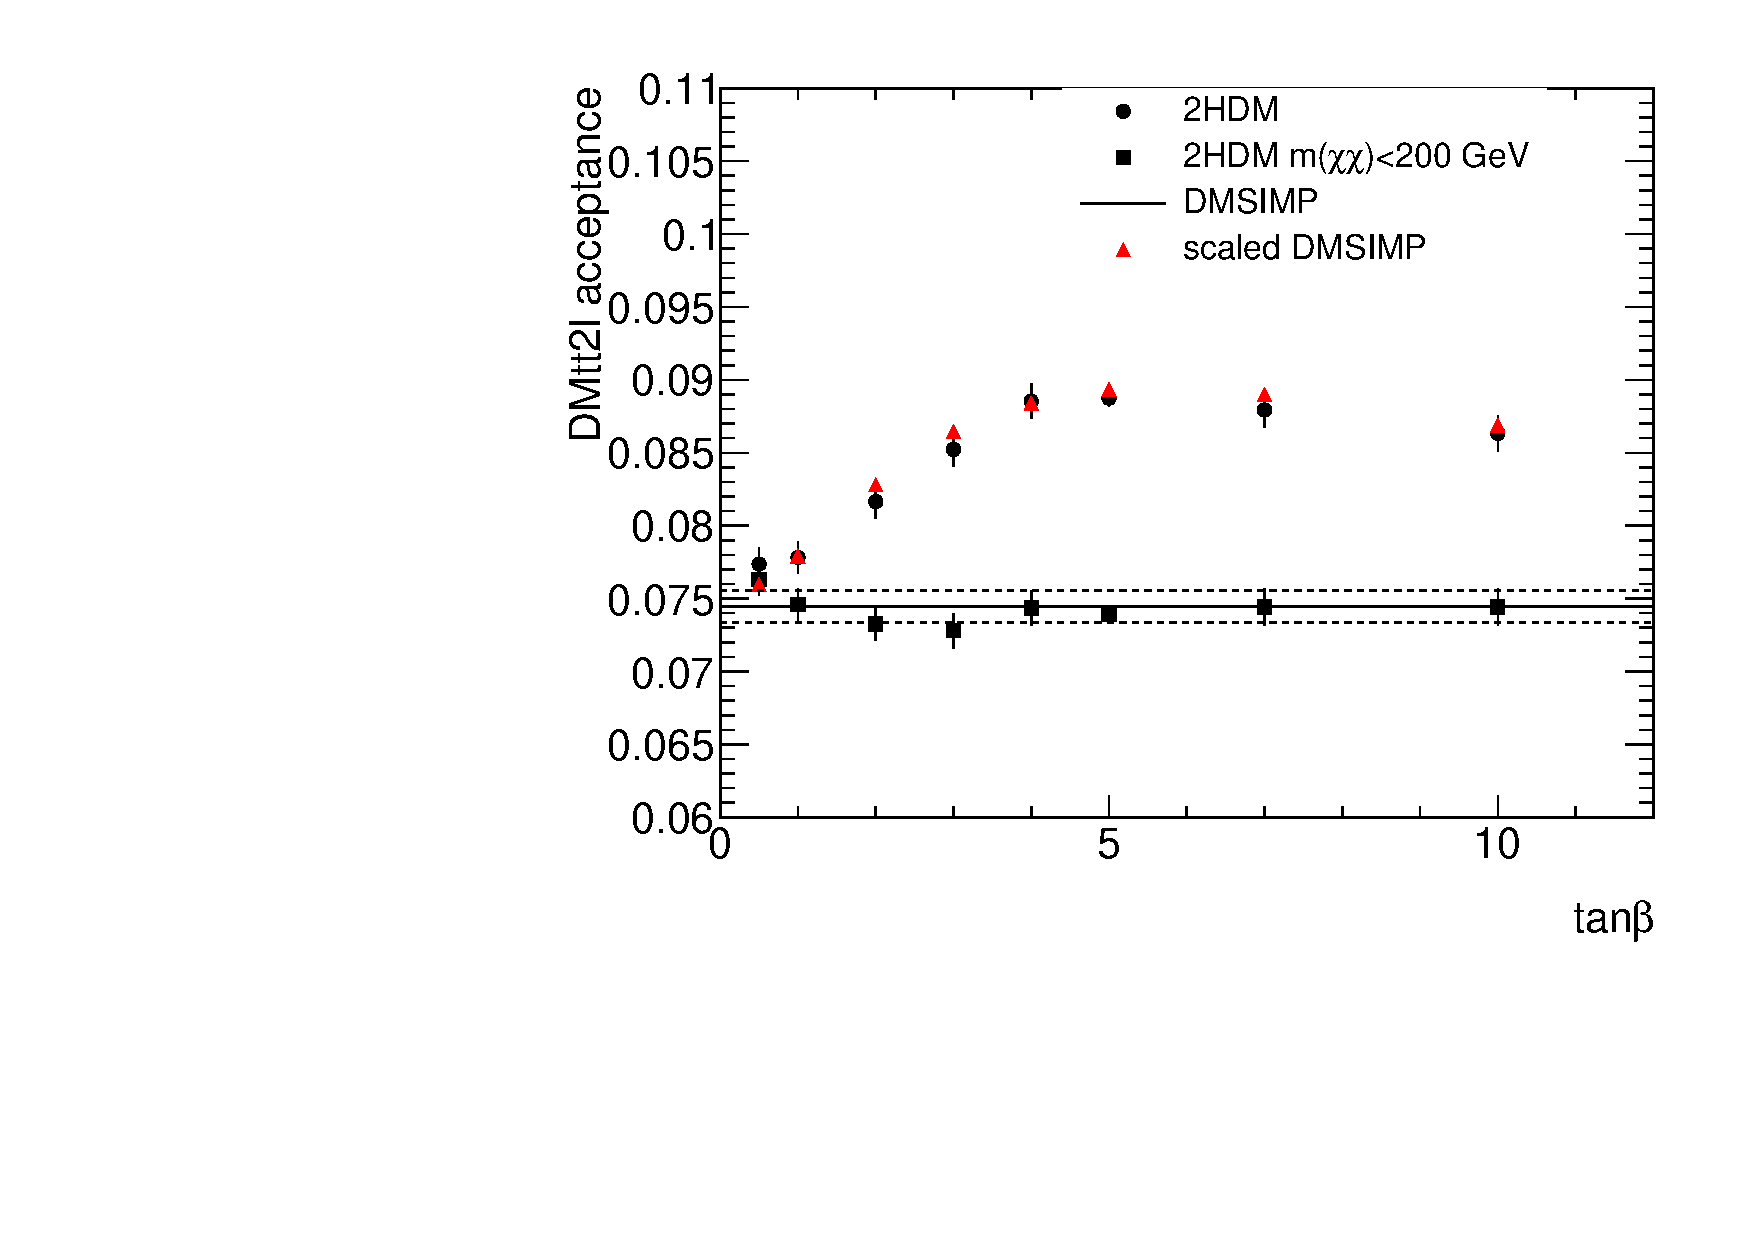
\includegraphics[width=0.7\textwidth]{texinputs/04_grid/figures/DMHF/plotacc_tb.pdf}
\caption{Acceptance of the two-lepton analysis as a function of $\tan\beta$ for the $2HDMp$ model (round markers), for the $2HDMp$ model considering only events with $m(\chi\chi)<200$~GeV (square markers), and for the \texttt{DMSimp} model (full line) for a mediator mass of 150~GeV. 
The two dashed lines indicate the statistical error of the \texttt{DMSimp}. The value of $m(A)$ is fixed at 600~GeV, and $\sin\theta=0.35$. 
The acceptance calculated from the \texttt{DMSimp} acceptance rescaled following the prescription in \autoref{eq:rew} (red triangles) is also shown.}
\label{fig:tbfin}
\end{center}
\end{figure}

%appendix
%\begin{figure}
%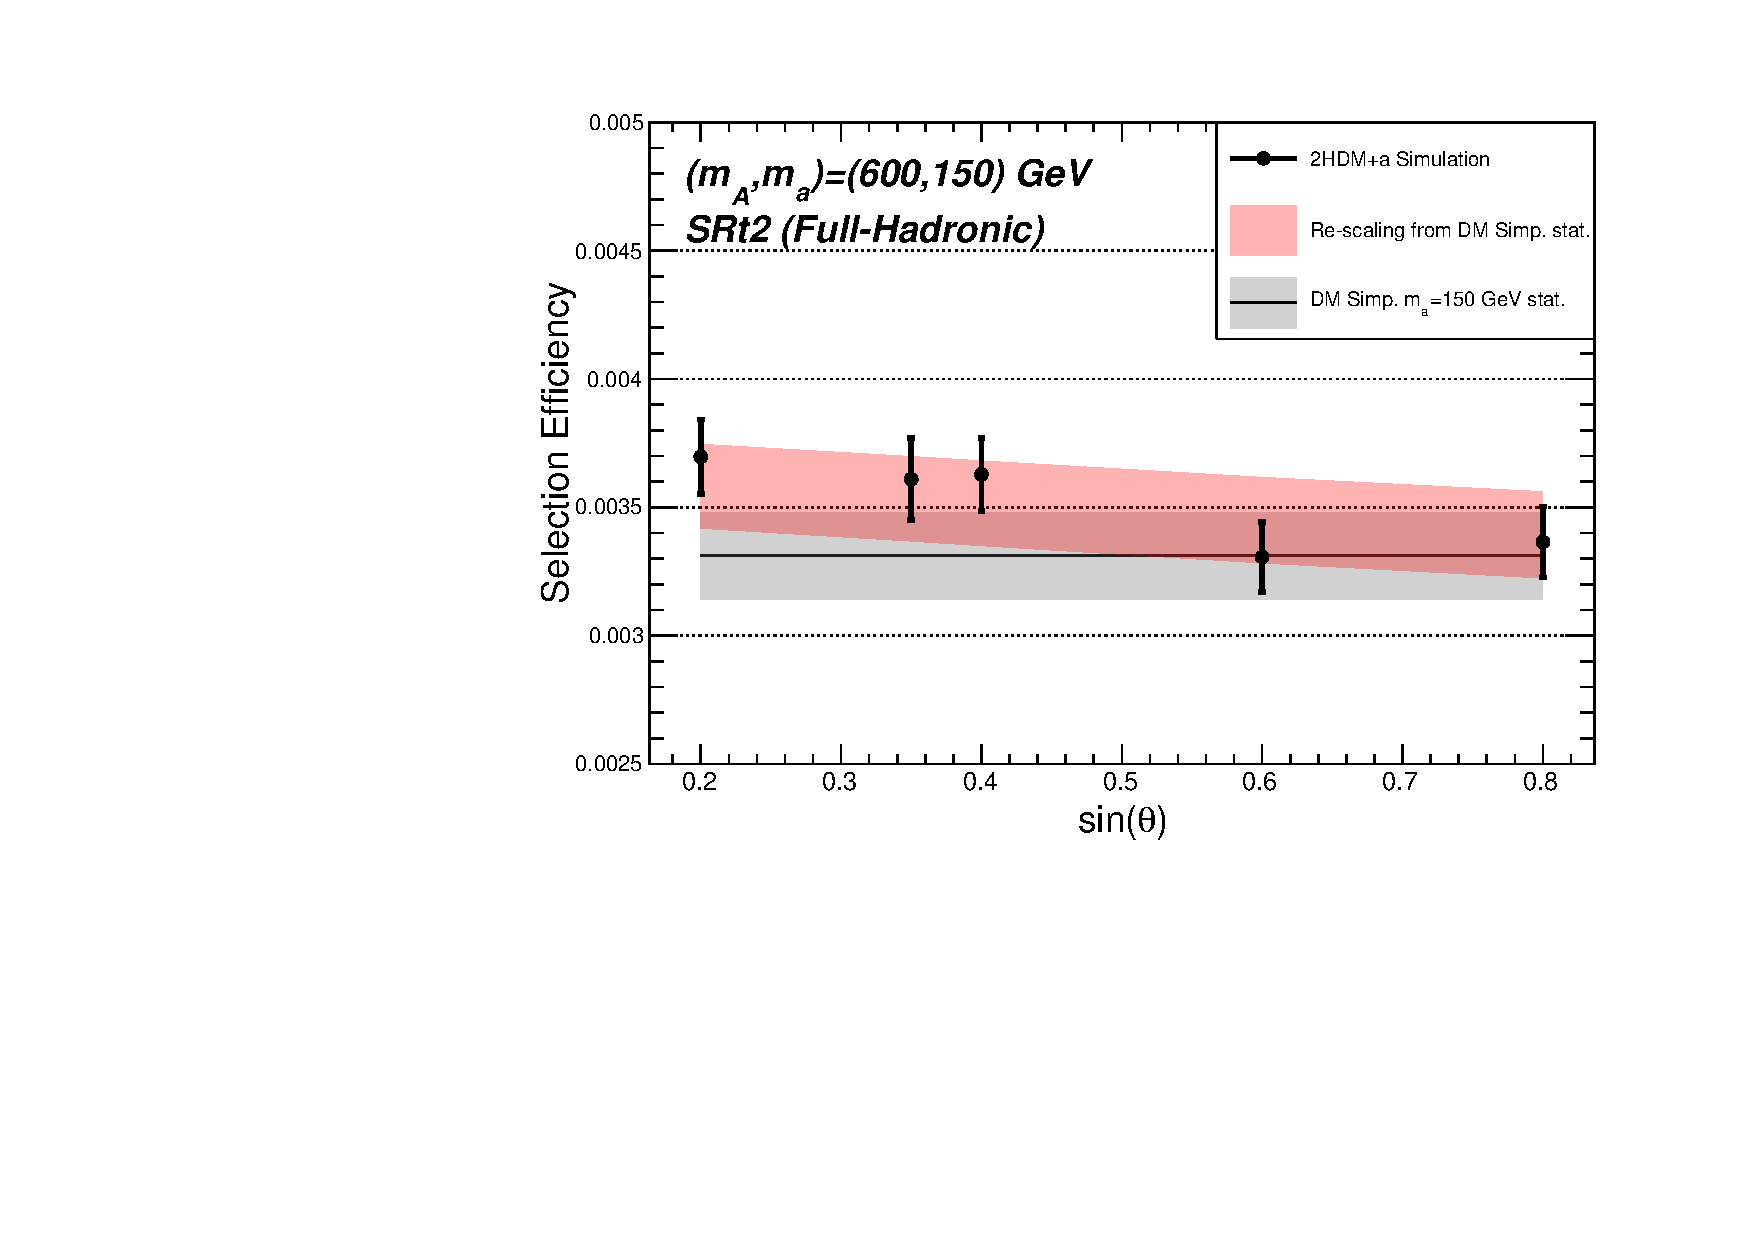
\includegraphics[width=.5\textwidth]{texinputs/04_grid/figures/DMHF/SRt2_600_150_sin}
%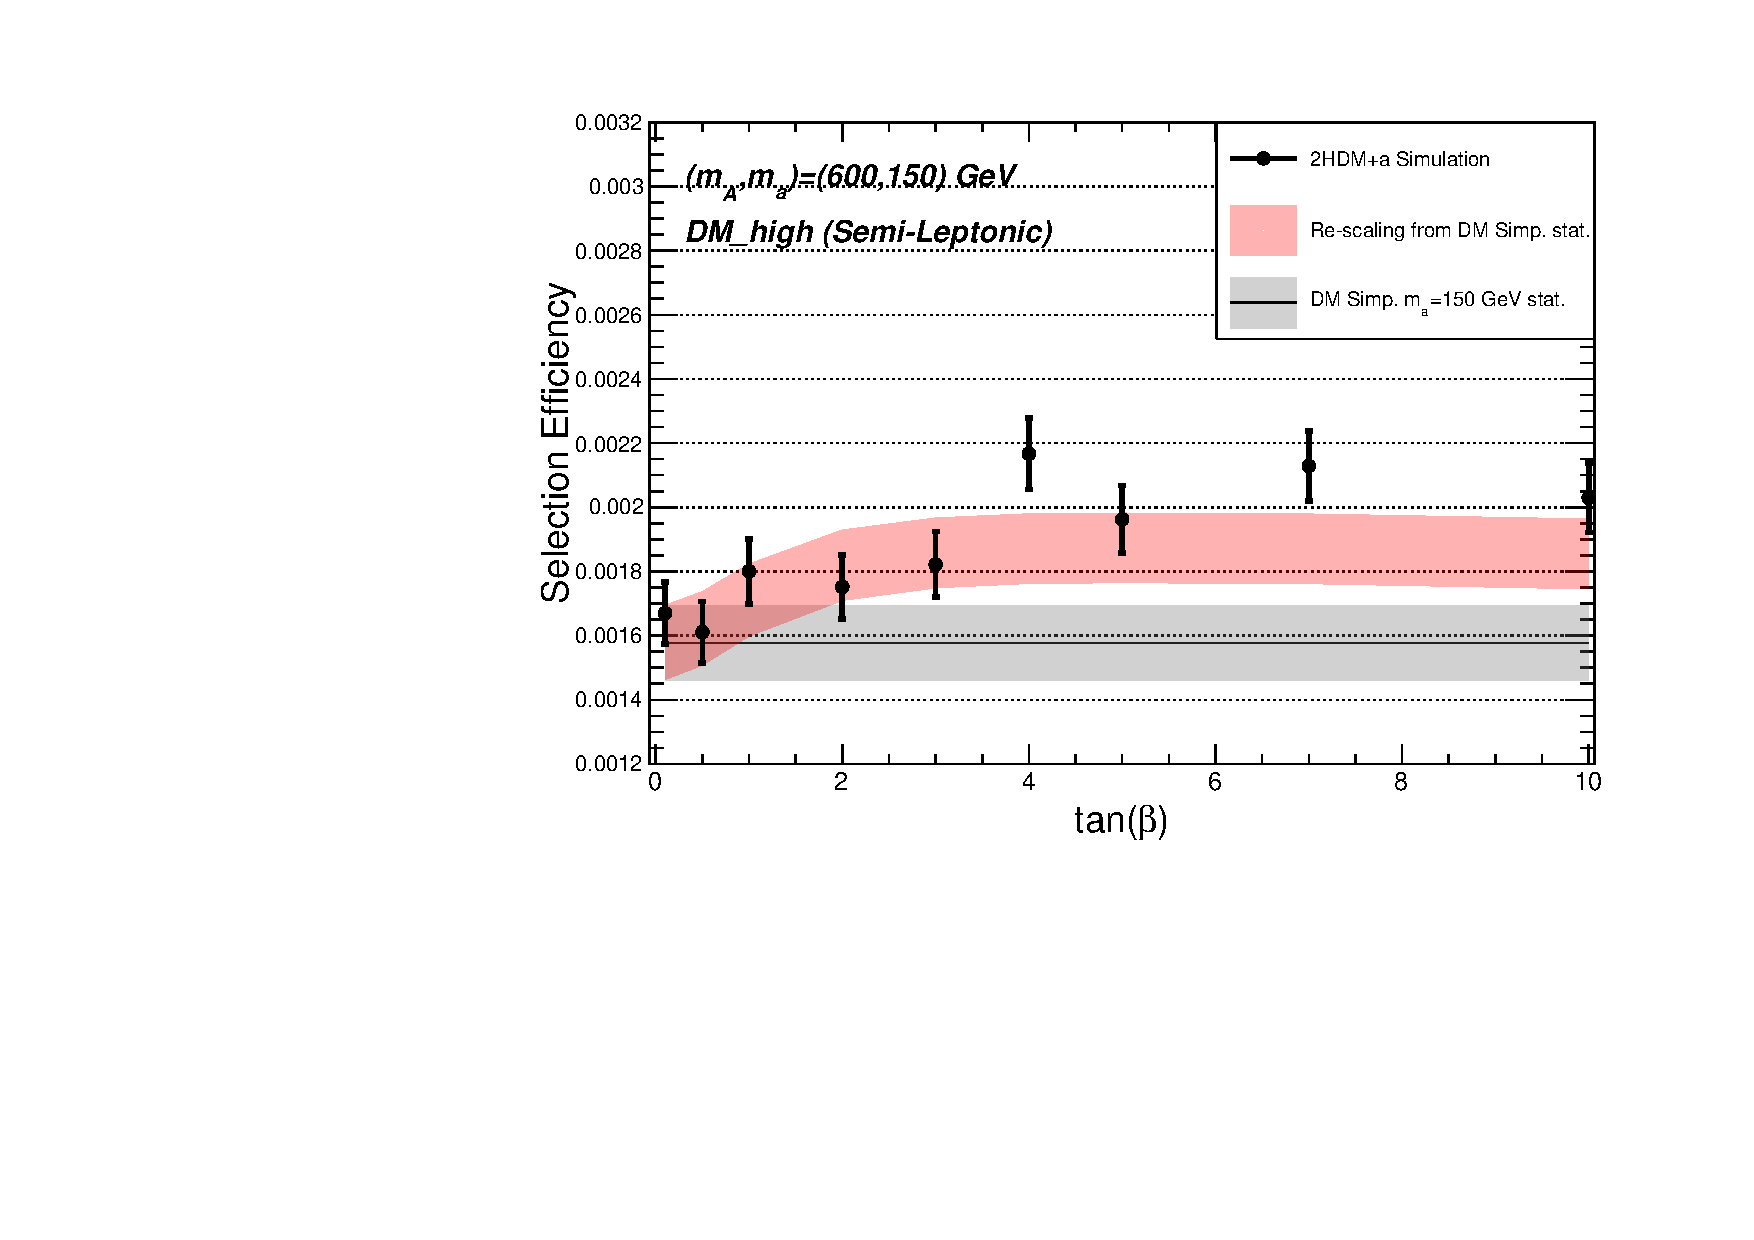
\includegraphics[width=.5\textwidth]{texinputs/04_grid/figures/DMHF/DM_high_600_150_tan}
%\caption{Validation of the re-scaling formula on zero and one lepton final states as a function of $tan\beta$ and $sin\theta$ parameters}
%\label{DMHF:pof}
%\end{figure}